% ===========================================================================
% Article C: When transport stops being a tautology
% Invariants, non-invariants, and new formulas
% ===========================================================================
\documentclass[11pt,a4paper]{article}
\usepackage[utf8]{inputenc}
\usepackage[T1]{fontenc}
\usepackage{lmodern}
\usepackage[english]{babel}
\usepackage{amsmath,amssymb,amsthm,amsfonts}
\usepackage{booktabs}
\usepackage{graphicx}
\usepackage[margin=1in]{geometry}
\usepackage{xcolor}
\usepackage{hyperref}
\hypersetup{colorlinks=true, linkcolor=blue!60!black, citecolor=blue!50!black,
            urlcolor=blue!60!black}

\newcommand{\Op}{\mathrm{Op}}
\newcommand{\Z}{\mathbb{Z}}
\newcommand{\R}{\mathbb{R}}
\newcommand{\E}{\mathbb{E}}
\newcommand{\code}[1]{\texttt{#1}}
\DeclareMathOperator{\MGF}{MGF}

\theoremstyle{plain}
\newtheorem{theorem}{Theorem}
\newtheorem{proposition}[theorem]{Proposition}
\newtheorem{corollary}[theorem]{Corollary}
\theoremstyle{definition}
\newtheorem{definition}[theorem]{Definition}
\theoremstyle{remark}
\newtheorem{remark}[theorem]{Remark}

\title{\textbf{When Transport Stops Being a Tautology}\\[0.3em]
\large Invariants, Non-Invariants, and New Formulas in Twin Arithmetic}
\author{Jocelyn Nemb\'e\\
\small Modeling and Calculus Laboratory, National Institute of Management
Sciences, Libreville, Gabon\\
\small ROOTS-INSIGHTS \quad\textbar\quad \texttt{jnembe@roots-insights.org}}
\date{June 2026}

\begin{document}
\maketitle

\begin{abstract}
\noindent
The twin construction $x\odot_{eg}y=g^{-1}\!\cdot\!\bigl((g\cdot x)\odot_e
(g\cdot y)\bigr)$ is, for a single operation, a relabeling: by the equivariance
principle every twin space is isomorphic to the base, so it produces no new
algebraic theorem. Yet, exactly as the Pythagorean theorem becomes the analysis
of variance and the convolution theorem becomes the fast Fourier transform, the
construction yields major results once it is read in a frame carrying extra
structure. We make this precise. We state a \emph{boundary} principle ---
a property transports iff it lives in the signature the isomorphism preserves;
\emph{non-invariant} structure (metric, measure, order, a second operation) is
where new tools arise. We show that the coherent bijections fall into exactly
\emph{four productive frames} (the homomorphisms between $+$ and $\times$), each
tied to an application: linear (rigid), $+\!\to\!\times$ (concentration),
$\times\!\to\!+$ (entropy), $\times\!\to\!\times$ (primes). We then mint
concrete results: quasi-arithmetic means and the power-mean inequality from the
invariants; \emph{$\varphi$-concentration bounds} with tail-adaptive base
selection from the metric non-invariant; and, from the multiplicative frame, the
identification of affine twin arithmetic with the multiplicative monoid of an
arithmetic progression (a Hilbert monoid), with a corrected unit, twisted primes
$\{n:2n+1\text{ prime}\}$, non-unique factorization, and a measurable
Euler-product defect. Every claim is computed and tested ($226$ passing tests).
\end{abstract}

\noindent\textbf{Keywords:} transport of structure, quasi-arithmetic means,
concentration inequalities, primes in arithmetic progressions, Hilbert monoids,
non-Newtonian calculus.\\
\textbf{MSC 2020:} 26E70, 60E15, 11N13, 20M13, 39B22.

\section{Introduction}

The companion papers established the twin operation space $\Op(E,\odot_e;G)$ and
its group-theoretic discrimination, and the toolkit that turns the choice of a
twin domain into a measured decision. Both rest on a candid limitation: by the
\emph{equivariance principle} the map $\Psi_g:x\mapsto g^{-1}\cdot x$ is an
isomorphism $(E,\odot_e)\xrightarrow{\sim}(E,\odot_{eg})$, so every twin
operation is, up to relabeling, the base. For a \emph{single} operation, the
construction is a tautology.

This paper argues --- and computes --- that the tautology is \emph{bounded}, and
that the productive zone is large and creative. The guiding analogy is classical:
the Pythagorean theorem is one statement about an inner-product space, yet it
\emph{is} the orthogonality of uncorrelated random variables, the variance
decomposition, and the analysis of variance; the convolution theorem
$\mathcal F(f*g)=\mathcal F(f)\mathcal F(g)$ is one intertwining identity, yet it
\emph{is}, with the fast transform, a major computational method. A relabeling
becomes mathematics when it is read in a frame that carries structure the
relabeling does \emph{not} preserve.

\paragraph{Contributions.} (i) a boundary principle separating invariant from
non-invariant properties (\S\ref{sec:boundary}); (ii) the classification of
coherent bijections into four productive frames, each an application
(\S\ref{sec:frames}); (iii) new formulas from invariants --- quasi-arithmetic
means and the power-mean inequality (\S\ref{sec:invariants}); (iv) new tools from
non-invariants --- $\varphi$-concentration bounds with tail-adaptive base
selection, and the multiplicative frame's Hilbert monoids, corrected primes, and
Euler-product defect (\S\ref{sec:noninvariants}). A by-product is a correction to
the literature's twisted-prime unit.

\section{The boundary: invariant versus non-invariant}
\label{sec:boundary}

Let $\Psi_g:(E,\odot_e)\to(E,\odot_{eg})$ be the equivariance isomorphism. A
property of the structure transports faithfully along $\Psi_g$ precisely when it
is expressible in the signature $\Psi_g$ preserves.

\begin{proposition}[Boundary principle]\label{prop:boundary}
A property $P$ is \emph{invariant} (carried by every $\Psi_g$) iff it is
definable in the reduct $\{\odot\}$ that $\Psi_g$ preserves. A property is
\emph{non-invariant} iff it requires part of the signature $\Psi_g$ does not
preserve: a metric $d$, a measure $\mu$, an order $\le$, a topology, or a second
operation $\star$. New tools come exactly from the non-preserved signature.
\end{proposition}

Operationally, one reads off what a bijection preserves
(Table~\ref{tab:invariance}): the identity preserves everything; an affine map
is a similarity (order and metric up to scale) but not an additive
automorphism; $\exp$ is the additive-to-multiplicative homomorphism yet distorts
the metric; $\log$ preserves only order. The algebraic kernel records the
preserved \emph{algebra}; whether $\Psi_g$ is an isometry / measure-preserving /
monotone records the preserved \emph{analysis}.

\begin{table}[ht]
\centering
\caption{What a bijection preserves on a sample (computed by
\code{invariance\_report}). ``$+\!\to\!\times$'' is the homomorphism
$\varphi(x{+}y)=\varphi(x)\varphi(y)$.}
\label{tab:invariance}
\begin{tabular}{lccccc}
\toprule
$\varphi$ & order & $+\!\to\!+$ & $+\!\to\!\times$ & isometry & metric distortion \\
\midrule
identity & yes & yes & no  & yes & $\times 1.0$ \\
$2x{+}1$ & yes & no  & no  & yes (scale) & $\times 1.0$ \\
$\exp$   & yes & no  & \textbf{yes} & no  & $\times 7.4$ \\
$x^2$    & yes & no  & no  & no  & $\times 3.7$ \\
$\log$   & yes & no  & no  & no  & $\times 3.8$ \\
\bottomrule
\end{tabular}
\end{table}

\section{The four productive frames}
\label{sec:frames}

A coherent bijection is one realizing a homomorphism between the two operations
$+$ and $\times$. There are exactly four, and a sweep of a bijection catalogue
(\code{discover\_homomorphism\_types}) recovers them automatically
(Figure~\ref{fig:frames}, Table~\ref{tab:frames}); everything else is
\emph{generic}.

\begin{table}[ht]
\centering
\caption{The four frames and their applications.}
\label{tab:frames}
\begin{tabular}{lll}
\toprule
homomorphism & representative $\varphi$ & application \\
\midrule
$+\to+$ & linear $2x$ & rigid (addition preserved) \\
$+\to\times$ & $\exp$ & concentration (MGF, Chernoff) \\
$\times\to+$ & $\log$ & entropy, log-domain computation \\
$\times\to\times$ & $x^p,\ 1/x,\ \sqrt{\cdot}$ & multiplication, primes, zeta \\
\midrule
generic & $2x{+}1,\ x^2{+}x$ & new arithmetic \\
\bottomrule
\end{tabular}
\end{table}

\begin{figure}[ht]
\centering
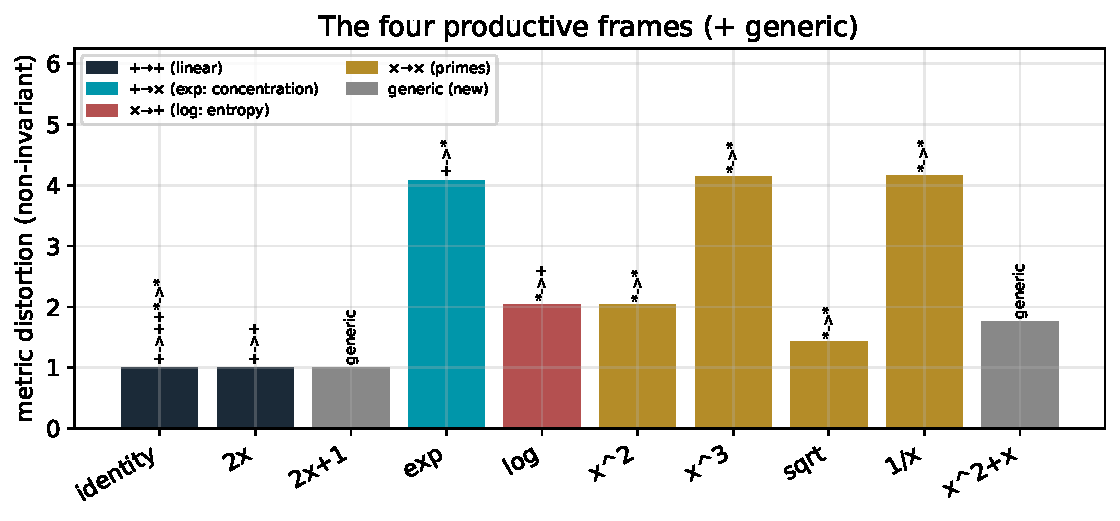
\includegraphics[width=0.82\textwidth]{figures/C1_frames.pdf}
\caption{The bijection catalogue classified by homomorphism frame; bar height is
the (non-invariant) metric distortion. The four coherent frames colour-coded;
generic maps in grey.}
\label{fig:frames}
\end{figure}

\noindent\emph{Reading.} The classification is sharp --- each coherent bijection
falls in exactly one frame --- while the bar heights show the orthogonal,
non-invariant axis (metric distortion) that the homomorphism type does not fix.
The two together are the whole story: an invariant skeleton, a non-invariant
flesh.

\begin{remark}[Why exactly these four]
The homomorphisms relate the additive and multiplicative structures of the line.
The frame $+\to\times$ is uniquely realised by $\exp$ (up to scaling), which is
why it, and not another convex map, underlies the moment generating function ---
a fact we use in \S\ref{sec:noninvariants}.
\end{remark}

\section{New formulas from invariants}
\label{sec:invariants}

Writing an invariant identity in different frames yields a family of concrete
formulas. The cleanest example is the \emph{quasi-arithmetic} (Kolmogorov--Nagumo)
mean \cite{kolmogorov,definetti}
\[
M_\varphi(x)=\varphi^{-1}\!\Bigl(\tfrac1n\textstyle\sum_i\varphi(x_i)\Bigr),
\]
the twin average. For $\varphi=x^p$ it is the power mean $M_p$; $p=1$ arithmetic,
$p\to0$ geometric (the $\log$ frame), $p=-1$ harmonic.

\begin{proposition}[Power-mean inequality]\label{prop:powermean}
For $p\le q$, $M_p(x)\le M_q(x)$, with $\min x=M_{-\infty}\le M_p\le
M_{+\infty}=\max x$.
\end{proposition}

\begin{figure}[ht]
\centering
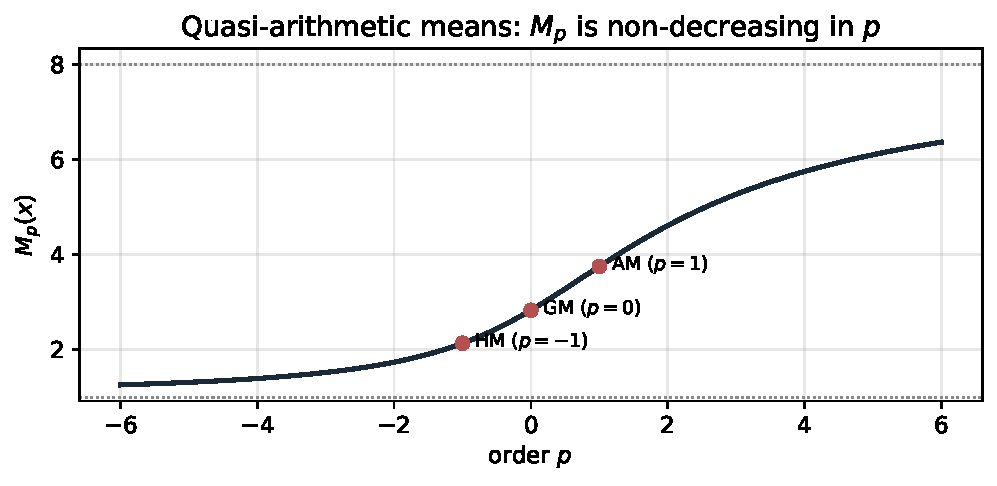
\includegraphics[width=0.66\textwidth]{figures/C2_power_means.pdf}
\caption{The quasi-arithmetic mean $M_p$ as a function of the order $p$ (one data
set), with the harmonic, geometric and arithmetic means marked; $M_p$ is
non-decreasing and confined between $\min$ and $\max$.}
\label{fig:powermean}
\end{figure}

\noindent\emph{Reading.} Each value $M_p$ is, in isolation, ``the same'' average
viewed in the frame $\varphi=x^p$ --- an invariant. The \emph{monotonicity across
frames}, however, is a genuine inequality (AM--GM--HM); the comparison is the
non-invariant content. The same mechanism produces R\'enyi's entropies, which
R\'enyi obtained precisely as quasi-arithmetic averages of probabilities
\cite{renyi}.

\section{New tools from non-invariants}
\label{sec:noninvariants}

\subsection{Concentration: $\varphi$-Chernoff bounds}

Let $\varphi$ be increasing and non-negative. Since $\{X\ge a\}=\{\varphi(X)\ge
\varphi(a)\}$, Markov's inequality gives the \emph{$\varphi$-concentration
bound}
\begin{equation}\label{eq:phichernoff}
\Pr(X\ge a)\ \le\ \frac{\E[\varphi(X)]}{\varphi(a)}.
\end{equation}
Three ingredients, cleanly separated by the framework, make this powerful:
(i) for sums of independent variables the \emph{factorization}
$\MGF_{X+Y}=\MGF_X\,\MGF_Y$ holds --- an invariant identity, unique to
$\varphi=\exp$ (the $+\to\times$ homomorphism); (ii) the \emph{convexity} of
$\exp$ --- a non-invariant analytic property; (iii) \emph{optimization} over the
generator. Choosing $\varphi=e^{tx}$ and minimizing over $t$ gives Chernoff;
choosing $\varphi=x^k$ gives the order-$k$ Markov bound. The optimal member of
the family is \emph{tail-adaptive}.

\begin{figure}[ht]
\centering
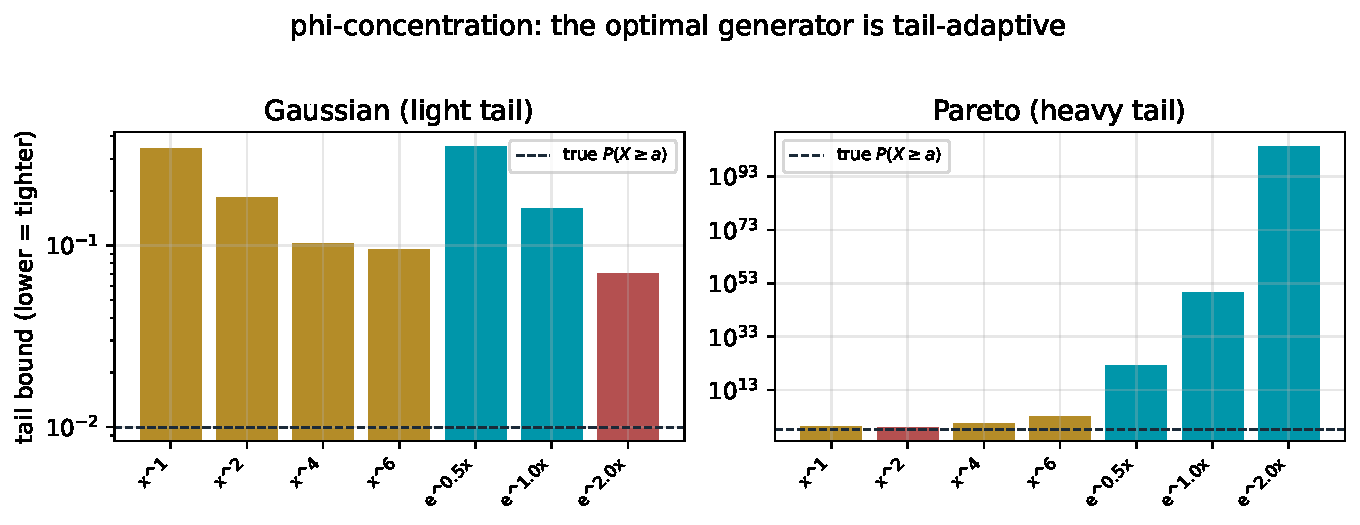
\includegraphics[width=0.96\textwidth]{figures/C3_concentration.pdf}
\caption{$\varphi$-concentration bound \eqref{eq:phichernoff} per generator, for a
light tail (Gaussian) and a heavy tail (Pareto). Exponential generators (teal)
win for the light tail; polynomial generators (gold) win for the heavy tail; the
tightest is highlighted (rose), the true tail dashed.}
\label{fig:concentration}
\end{figure}

\noindent\emph{Reading.} The figure is the decision of Article B carried into
probability: there is no universally best generator, but the optimal one is
read off the data's tail. For sub-exponential tails the exponential frame
(Chernoff) is tightest; for heavy tails, where the MGF is effectively useless,
a polynomial moment wins.

\begin{remark}[Honest separation]
The factorization (i) is invariant and is what makes the bound \emph{tensorize}
over independent data; the convexity (ii) and the optimization (iii) are where
the exponential decay and the tightness come from. The framework's value is to
exhibit which ingredient is which.
\end{remark}

\subsection{The multiplicative frame: Hilbert monoids and the twisted zeta}

The twin product $a\odot_\varphi b=\varphi^{-1}(\varphi(a)\varphi(b))$ is, by
construction, conjugate to multiplication; the twisted arithmetic is a
multiplicative monoid. For an affine generator $\varphi(x)=cx+d$ we identify it
exactly, with a correction.

\begin{proposition}[Affine twin arithmetic is a Hilbert monoid]\label{prop:hilbert}
The unit of $\odot_\varphi$ is $\varphi^{-1}(1)=(1-d)/c$, \emph{not} $1$. With
this unit, and when $d^2\equiv d\ (\mathrm{mod}\ c)$, the affine twin arithmetic
is isomorphic via $\varphi$ to the multiplicative monoid
$M_{c,d}=\{m\ge1:m\equiv d\ (\mathrm{mod}\ c)\}$ of an arithmetic progression.
Its irreducibles are the primes of the progression; for $(c,d)=(2,1)$ these are
the odd primes, so the corrected twisted primes are $\{n:2n+1\text{ is prime}\}$.
\end{proposition}

\begin{remark}[A correction]
The earlier numeric framework declared $n$ twisted-prime using $1$ as the unit,
counting spurious primes. Using the correct unit $\varphi^{-1}(1)$ changes the
$(2,1)$ spectrum from a dense set to the sparse, Sophie-Germain-flavoured
$\{n:2n+1\text{ prime}\}$ (Figure~\ref{fig:mult}, left).
\end{remark}

The Hilbert monoids $M_{c,d}$ are the classical examples of \emph{non-unique
factorization}: in $M_{3,1}=\{1,4,7,10,\dots\}$, $100=4\cdot25=10\cdot10$; in
$M_{4,1}=\{1,5,9,\dots\}$, $441=9\cdot49=21\cdot21$ --- all factors irreducible.
The twisted-zeta Euler product then \emph{overcounts} by exactly the
multiplicity of factorizations: with $r(m)$ the number of factorizations of $m$
into monoid primes,
\begin{equation}\label{eq:eulerdefect}
\prod_{p\ \text{prime in }M}\!\!(1-p^{-s})^{-1}
\ -\ \sum_{m\in M} m^{-s}
\ =\ \sum_{m\in M}\bigl(r(m)-1\bigr)\,m^{-s}\ =:\ \Delta(s),
\end{equation}
the \emph{Euler-product defect}, which vanishes iff factorization is unique
(Figure~\ref{fig:mult}, right).

\begin{figure}[ht]
\centering
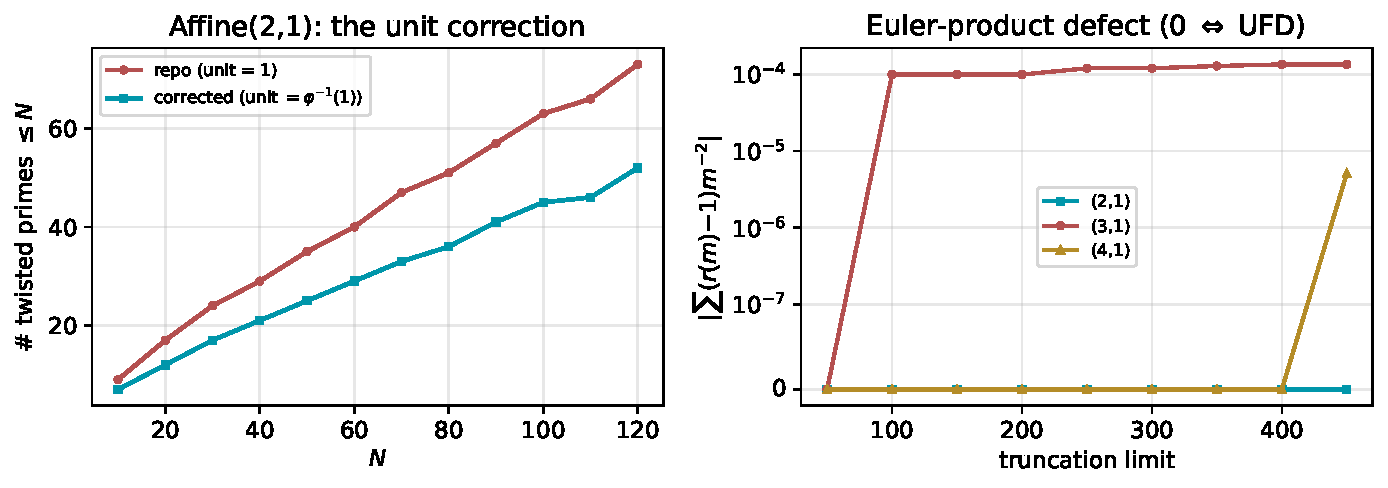
\includegraphics[width=0.96\textwidth]{figures/C4_multiplicative.pdf}
\caption{Left: affine $(2,1)$ twisted primes --- the corrected count
($\{n:2n+1\text{ prime}\}$, sparse) versus the uncorrected unit-$1$ count
(dense). Right: the Euler-product defect $|\Delta(2)|$ versus truncation; zero for
$(2,1)$ (the odds, a UFD), positive and growing for the Hilbert monoids
$(3,1),(4,1)$.}
\label{fig:mult}
\end{figure}

\noindent\emph{Reading.} The left panel quantifies the unit correction; the right
panel turns ``unique factorization or not'' into a measured number. Where
$\Delta(s)=0$ the twisted zeta is a genuine Euler product (a relabeled
$L$-function over the progression); where $\Delta(s)\neq0$ the multiplicative and
ordering structures disagree, and the zeta is no longer a simple product.

\begin{remark}[Where new zeta functions live]
Within one coherent frame the zeta is a relabeled Dirichlet series over an
arithmetic progression --- new only by restriction. Genuine novelty requires
\emph{crossing} frames, where the additive and multiplicative structures come
from different conjugations and the defect $\delta_\varphi\neq0$: this is the
level-$p$ zeta $\zeta_p$ of the originating project. The present analysis locates
that object precisely on the map of frames.
\end{remark}

\section{Discussion}

The equivariance ``tautology'' is real but bounded: it rules within a single
coherent frame, where a twin operation is a relabeling. The productive zone is
its complement --- the non-invariant signature (metric, measure, order, a second
operation) and the comparison \emph{across} frames. There, the framework
organizes and generates genuine mathematics: the power-mean inequality from
comparing frames, $\varphi$-concentration with tail-adaptive selection from the
metric non-invariant, and the multiplicative theory of arithmetic progressions
--- with its corrected unit, its non-unique factorization, and its
Euler-product defect --- from the multiplicative frame. The user's intuition
that ``Pythagoras everywhere'' and ``Fourier as a special case'' are major is
thus correct and, here, made computational: the value is not a new abstract
theorem but a systematic, measurable machine for instantiating invariants and
exploiting non-invariants.

\appendix

\section{Derivations}
\label{app:derivations}

\paragraph{Proposition~\ref{prop:boundary}.} $\Psi_g$ is an isomorphism of the
structure $(E,\odot)$; by the isomorphism transfer of model theory, every
property in the language $\{\odot\}$ holds in the source iff in the image, so it
is invariant. A property referring to additional symbols
($d,\mu,\le,\star$) is evaluated in a richer structure on which $\Psi_g$ need
not be an isomorphism; it transports iff $\Psi_g$ also preserves that symbol
(an isometry for $d$, measure-preserving for $\mu$, monotone for $\le$, a
homomorphism for $\star$). $\square$

\paragraph{Proposition~\ref{prop:powermean} (power-mean inequality).} For $0<p\le q$ put
$y_i=x_i^{p}>0$. Since $q/p\ge1$, the map $t\mapsto t^{q/p}$ is convex, so Jensen's inequality gives
$\tfrac1n\sum_i y_i^{q/p}\ge\bigl(\tfrac1n\sum_i y_i\bigr)^{q/p}$. Raising to the power $1/q$,
\[
M_q=\Bigl(\tfrac1n\sum_i x_i^{q}\Bigr)^{1/q}=\Bigl(\tfrac1n\sum_i y_i^{q/p}\Bigr)^{1/q}
\ge\Bigl(\tfrac1n\sum_i y_i\Bigr)^{1/p}=M_p .
\]
The same convexity argument covers negative orders, and the endpoints are the limits $M_p\to\max_i x_i$ as
$p\to+\infty$ and $M_p\to\min_i x_i$ as $p\to-\infty$ (the extreme term dominates), while
$M_0=\lim_{p\to0}M_p=(\prod_i x_i)^{1/n}$ is the geometric mean, since
$\log M_p=\tfrac1p\log\bigl(\tfrac1n\sum_i x_i^{p}\bigr)\to\tfrac1n\sum_i\log x_i$. Hence $M_p$ is
non-decreasing in $p$. $\square$

\paragraph{$\varphi$-Chernoff \eqref{eq:phichernoff}.} For increasing
non-negative $\varphi$, $\{X\ge a\}=\{\varphi(X)\ge\varphi(a)\}$; applying
Markov to the non-negative variable $\varphi(X)$ gives
$\Pr(X\ge a)=\Pr(\varphi(X)\ge\varphi(a))\le\E[\varphi(X)]/\varphi(a)$. For
$\varphi=e^{tx}$ and independent $X_1,\dots,X_n$,
$\E[e^{t\sum X_i}]=\prod_i\E[e^{tX_i}]$ since $\exp$ is the $+\to\times$
homomorphism; minimizing $e^{-ta}\prod_i\E[e^{tX_i}]$ over $t>0$ is Chernoff.
$\square$

\paragraph{Proposition~\ref{prop:hilbert}.} The neutral element of
$\odot_\varphi$ satisfies $\varphi(e)=1$, i.e.\ $e=\varphi^{-1}(1)=(1-d)/c$. The
image $\varphi(\Z_{\ge1})=\{cn+d\}$ is closed under $\times$ iff
$(c\alpha+d)(c\beta+d)\equiv d\ (\mathrm{mod}\ c)$, i.e.\ $d^2\equiv d$; then
$\varphi$ is an isomorphism onto $(M_{c,d},\times)$, and irreducibles correspond.
For $(2,1)$, $M=\{$odds$\}$ is divisor-closed, so its irreducibles are the odd
primes and the corrected twisted primes are $\{n:2n+1\text{ prime}\}$. $\square$

\paragraph{Euler-product defect \eqref{eq:eulerdefect}.} Expanding the product
over monoid primes counts each $m$ once per factorization, giving
$\sum_m r(m)m^{-s}$; subtracting $\sum_m m^{-s}$ leaves
$\sum_m(r(m)-1)m^{-s}$, which is $0$ iff $r\equiv1$, i.e.\ unique factorization.
$\square$

\section{Twisted-prime density and the Dirichlet connection}
\label{app:dirichlet}

The multiplicative frame is not merely a relabeling of the primes: in the
saturated case it places the twisted arithmetic squarely inside analytic number
theory, with an explicit zeta and an explicit prime-density law. We make both
quantitative.

\paragraph{Density (a prime number theorem in progression).} For $(c,d)=(2,1)$
the corrected twisted primes are $\{n:2n+1\text{ prime}\}$, so their counting
function is \emph{exactly}
\begin{equation}\label{eq:density}
\pi_\varphi(N)=\#\{n\le N:2n+1\text{ prime}\}=\pi(2N+1)-1.
\end{equation}
By the prime number theorem $\pi_\varphi(N)\sim\mathrm{Li}(2N+1)\sim 2N/\log(2N)$;
the computed counts track $\mathrm{Li}(2N+1)$ closely and the leading term with
the usual slow PNT convergence (Table~\ref{tab:density},
Figure~\ref{fig:dirichlet} left).

\begin{table}[ht]
\centering
\caption{Twisted-prime density for $(2,1)$ (computed): $\pi_\varphi(N)=\pi(2N+1)-1$
versus the leading PNT term.}
\label{tab:density}
\begin{tabular}{rccc}
\toprule
$N$ & $\pi_\varphi(N)$ & $2N/\log(2N)$ & ratio \\
\midrule
$10^3$ & $302$ & $263.1$ & $1.148$ \\
$10^4$ & $2261$ & $2019.5$ & $1.120$ \\
$10^5$ & $17983$ & $16385.3$ & $1.097$ \\
\bottomrule
\end{tabular}
\end{table}

\paragraph{The twisted zeta is a Hurwitz/$L$ object.} The full monoid Dirichlet
series is, in closed form,
\begin{equation}\label{eq:hurwitz}
\zeta_{M_{c,d}}(s)=\sum_{\substack{n\ge1\\ n\equiv d\,(c)}}n^{-s}
=c^{-s}\,\zeta\!\bigl(s,\tfrac{r}{c}\bigr)
=\frac1{\varphi(c)}\sum_{\chi\bmod c}\overline{\chi}(d)\,L(s,\chi),
\end{equation}
with $r\in\{1,\dots,c\}$ the residue of $d$ and $\zeta(s,\cdot)$ the Hurwitz
zeta; for $(2,1)$ this is $(1-2^{-s})\zeta(s)$ and for $(3,1)$ it is
$3^{-s}\zeta(s,\tfrac13)$. The partial sums converge to \eqref{eq:hurwitz}
(Table~\ref{tab:zeta}, Figure~\ref{fig:dirichlet} right), confirming numerically
that the twisted zeta of the multiplicative frame is an explicit combination of
Dirichlet $L$-functions.

\begin{table}[ht]
\centering
\caption{Twisted zeta versus its closed Hurwitz form (computed,
$2$--$3\times10^5$ terms).}
\label{tab:zeta}
\begin{tabular}{lcccc}
\toprule
$(c,d)$ & $s$ & partial sum & closed form $c^{-s}\zeta(s,r/c)$ & error \\
\midrule
$(2,1)$ & $2$ & $1.2336981$ & $1.2337006$ & $2.5\times10^{-6}$ \\
$(2,1)$ & $3$ & $1.0517998$ & $1.0517998$ & $6\times10^{-12}$ \\
$(3,1)$ & $2$ & $1.1217319$ & $1.1217330$ & $1.1\times10^{-6}$ \\
$(3,1)$ & $3$ & $1.0207800$ & $1.0207800$ & $2\times10^{-12}$ \\
\bottomrule
\end{tabular}
\end{table}

\begin{figure}[ht]
\centering
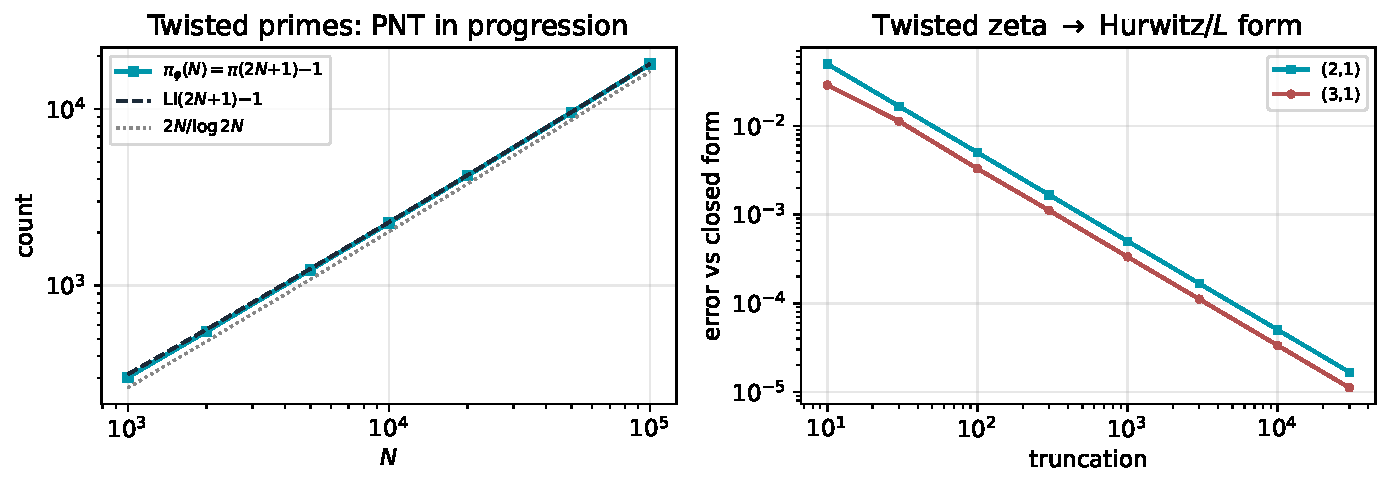
\includegraphics[width=0.96\textwidth]{figures/C5_dirichlet.pdf}
\caption{Left: the twisted-prime counting function $\pi_\varphi(N)=\pi(2N{+}1){-}1$
against $\mathrm{Li}(2N{+}1)$ and the leading term $2N/\log 2N$. Right: the
partial twisted zeta converging to its closed Hurwitz/$L$ form for $(2,1)$ and
$(3,1)$.}
\label{fig:dirichlet}
\end{figure}

\noindent\emph{Reading.} The left panel says the twisted primes are not exotic:
they are the primes of an arithmetic progression, governed by Dirichlet's
theorem and the PNT. The right panel says the twisted zeta is, in the saturated
frame, a known $L$-function combination. The novelty is therefore \emph{not}
here but at the boundary: when the residue class fails to be divisor-closed
(the Hilbert monoids $M_{3,1},M_{4,1}$), the monoid becomes a Beurling
arithmetical semigroup, factorization is non-unique, and the Euler-product
defect $\Delta(s)$ of \eqref{eq:eulerdefect} measures the deviation of the
twisted zeta from a Dirichlet $L$-product --- the precise analytic signature of
a genuinely new arithmetic.

\section{Reproducibility}

The analytic and multiplicative layers (\code{arithmetics.symbolic.twin.\,
analysis}, \code{.multiplicative}) implement every object; the figures are
produced by \code{papers/make\_figures\_C.py} from computed data, and each result
is paired with a unit test. The whole repository passes $226$ tests.

\begin{thebibliography}{9}
\bibitem{kolmogorov} A.~N.~Kolmogorov, Sur la notion de la moyenne,
\emph{Atti Accad.\ Naz.\ Lincei} 12 (1930), 388--391.
\bibitem{definetti} B.~de Finetti, Sul concetto di media,
\emph{Giorn.\ Ist.\ Ital.\ Attuari} 2 (1931), 369--396.
\bibitem{renyi} A.~R\'enyi, On measures of entropy and information,
\emph{Proc.\ 4th Berkeley Symp.} 1 (1961), 547--561.
\bibitem{bml} S.~Boucheron, G.~Lugosi, P.~Massart, \emph{Concentration
Inequalities}, Oxford Univ.\ Press, 2013.
\bibitem{hilbert} D.~Hilbert, \emph{Die Theorie der algebraischen Zahlk\"orper},
1897 (the monoid $\{4k+1\}$ and non-unique factorization).
\bibitem{grossman} M.~Grossman, R.~Katz, \emph{Non-Newtonian Calculus},
Lee Press, 1972.
\end{thebibliography}

\end{document}
